% !TEX root =  ../main_manuscript.tex 
\subsection{Statistical Methods}
The goal of the statistical analysis of the PRIAS data was to develop a model for predicting the time of reclassification. To this end, for each patient we have the information about his age at the start of AS, all observed PSA measurements, and the history of biopsies. Since PRIAS data is longitudinal in nature, the PSA measurements of a patient are correlated. PSA can be higher when measured closer to the time of reclassification. An additional complication is that such higher values are also often missing once a patient obtains reclassification. The vice versa, that is, reclassification is more likely when PSA increases is also plausible. A commonly used statistical method to model such complex correlation between a longitudinal outcome (PSA) and a time-to-event (reclassification) outcome is the joint model for time-to-event and longitudinal data \citep{rizopoulos2012joint,tomer2019,coley2017prediction}.

\begin{figure}[!htb]
\centerline{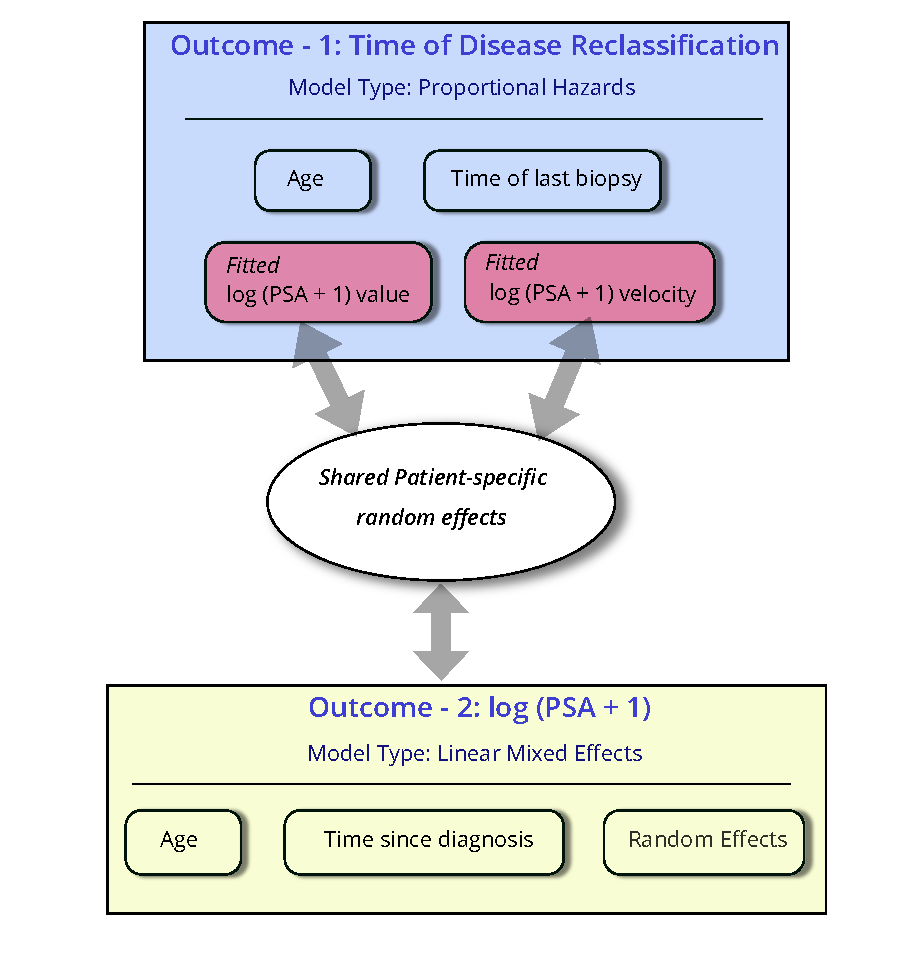
\includegraphics[width=\columnwidth]{images/jm_blockdiag.pdf}}
\caption{\textbf{Diagram of the joint model}: Per patient we observe the $\log_2\{\mbox{PSA + 1}\}$ transformed PSA, and the results of biopsies. We combine information from these observations to estimate the time of disease reclassification. To this end, we use a linear mixed effects model for $\log_2\{\mbox{PSA + 1}\}$ measurements, and proportional hazards model for time of disease reclassification. The time of disease reclassification depends on patient age, time of latest negative biopsy and underlying trend of PSA. To account for the correlation between PSA measurements and time of reclassification, the two models share patient-specific random effects in their model equations.}
\label{fig:jm_blockdiag}
\end{figure}

A joint model exploits patient-specific random effects (similar to random effects of a linear mixed effects model) to act as a common source of correlation between various outcomes (see Figure \ref{fig:jm_blockdiag}). These random effects manifest the unobservable patient-specific state of PCa. The joint model has separate sub-models for PSA and time of reclassification. However, both models utilize these random effects as covariates in the model. We used a linear mixed effects model for $\log_2\{\mbox{PSA + 1}\}$ transformed measurements, and a relative risk model (similar to cox model) for time of reclassification. The mixed effects model for PSA uses random effects to non-linearly model the evolution of PSA over time in a patient-specific manner. Simultaneously, in the relative risk model we establish the correlation between time of reclassification and PSA. This is achieved by using fitted $\log_2\{\mbox{PSA + 1}\}$ value and velocity as time dependent covariates, that is, random effects are used indirectly. Unlike observed $\log_2\{\mbox{PSA + 1}\}$ values, the fitted values are free of measurement errors. The $\log_2\{\mbox{PSA + 1}\}$ velocity is not modeled separately, but is rather mathematically derived as the rate of change of fitted $\log_2\{\mbox{PSA + 1}\}$ value over time. Since fitted $\log_2\{\mbox{PSA + 1}\}$ profiles are modeled non-linearly, the corresponding velocity is also allowed to change over follow-up. 

The various parameters of the two sub-models estimated jointly using the R \textbf{JMbayes} \citep{rizopoulosJMbayes}. This package utilizes the Bayesian methodology to estimate model parameters. The parameters and 95\% credible intervals are presented in Table.. of Appendix.

\subsection{Assessment of Predictions}
We assessed the goodness of fit of our model using both in-sample and out-of-sample predictions of reclassification. For out-of-sample predictions we utilized the five largest AS cohorts that constitute the GAP3 database \citep{gap3_2018}. We measured the accuracy of these predictions via two commonly used measures, namely the root mean squared prediction error (RMSPE) and the area under the receiver operating characteristic curve (AUC). Both of these measures take a value between zero and one. The RMSPE represents the difference between the true reclassification status of a patient, and the predicted risk of reclassification. Ideally the RMSPE should be zero. The AUC indicates if the model is able to discriminate between patients who obtain reclassification and those do not obtain it. Ideally it should be equal to one. In practice it should not be less than 0.5 (AUC of random discrimination). Since PRIAS is a longitudinal study, we compute these measures in a time dependent manner, at a gap of every one year until xx years of follow-up (95\% quantile of observed reclassification times).

\subsection{Estimate Risk of Reclassification and Consequences of Biopsies}
Consider a new patient with a certain history of biopsies, and PSA measurements. Using the joint model fitted to the PRIAS dataset, we first obtain his profile of the cumulative risk of reclassification over the follow-up period (Figure ...). We then suggest a biopsy at a follow-up visit if the cumulative risk at that visit is above a certain threshold (e.g. 10\% risk). The cumulative risk is updated at each new visit, by accounting for latest PSA measurements and decisions of biopsies. One can then repeatedly apply the threshold based decision rule for biopsies at each new visit. 

The choice of a threshold is not easy. To this end, we exploit the entire cumulative risk profile of a patient to estimate the consequences of following a particular threshold based schedule (Figure ...). The consequences we use in this paper are the expected delay in detection of reclassification, the corresponding number of biopsies required, at the estimated visit times at which they are scheduled. These estimates are patient specific and also updated with new data at each visit. Since we calculate the consequences for various fixed biopsy schedules as well, patients can make a more informed decision of biopsy. Lastly, we implemented this approach in a web-based application for use in medical centers.